% !TEX encoding = UTF-8
% !TEX TS-program = pdflatex
% !TEX root = ./thesis.tex
% !TEX spellcheck = en

%************************************************

One of the recognized problems in the web mining community  concerns the automatic construction of web pages hierarchies, typically called \emph{sitemaps}.
A sitemap represents an explicit specification of the design concept codified by User Experience Designers and Information Architects to define the knowledge organization of a website through grouping of related content \cite{Nielsen:2006}. This hierarchical organization of the content is coherent with the approach typically followed in the website navigation, where users start with the homepage or a web page found through a search engine or linked from another website, and then use the \emph{navigation systems}\footnote{A navigation system is a common set of hyperlinks implemented using similar layout which assist users during website's navigation (e.g. navbars, menus, product lists, etc.) \cite{Crescenzi:2005}.} provided by the website to find the desired information~\cite{Fang:2007}. %Studies reveal that users not randomly explore web pages in a website, but proceed in a top-down fashion, from a more general page to a detailed page using links of navigation systems with higher frequency compared to the other links of web graph~\cite{Anderson:2001,Amadieu:2010, Wang:2011, Weninger:2012}.  
Sitemaps help \emph{users} by: \emph{i)} increasing the user experience of a website; \emph{ii)} providing a complementary tool to the \emph{keyword-based search} for the information retrieval process.
In the first case, sitemaps organizing the website content in a top-down fashion, from a more general page to a detailed page, help users to understand, at glance, contextual information such as relationships among web pages (e.g. relationships of super/sub category), facilitates the discovery and the access of information and creates a better sense of orientation. %Sitemaps are particularly useful for websites with a great amount of contents and different types of visitors. In fact, in these cases embedded navigation systems are not able to codify every information needed for every visitor in every situation, whereas a sitemap could help.
In the second case, sitemaps help users when they do not know what they are looking for until the available options are presented or their information needs cannot be formulated in keywords~\cite{Lee:2005, Olston:2003}. In fact, in the keyword-based paradigm the search engine, given one or several key terms, returns an ordered list of web pages in descending order of relevance and accuracy. However, users have to express their information needs in form of keyword sequences which  should be as much discriminative as possible. For example, a sitemap can be useful in an university website to look for all professors or research areas. This kind of query is hard to answer by a search engine, but very simple to extract from a well designed sitemap.
%Moreover, by means of the automatic extraction of sitemaps, it is possible to extract the information asset of an organization, as it is available on its website, without access to the underlying organization's databases. 

Moreover, sitemaps help \emph{search engine bots} to extract the information asset of an organization, as it is available on its website, without access to the underlying organization's databases. For example, given an organization website, it is possible to discover all its affiliate companies, products, employees, etc. Finally, a sitemap can be used, in addition to the motivations reported before, also to improve existing applications like search engines integrating taxonomies in the presentation of search results~\cite{Keller:2013}, or to cluster web pages having same semantic type (e.g. web pages related to professors, courses, books, lists of publications of a single researchers)~\cite{Lin:2010b}. 

%Sitemaps are particularly useful for websites with a great amount of contents and different types of visitors. In fact, in these cases embedded navigation systems are not able to codify every information needed for every visitor in every situation, whereas a sitemap could help. In this view, sitemaps can be used, in addition to motivations reported before, also to improve existing applications like search engines, to create new applications that integrate taxonomies in the presentation of search results~\cite{Keller:2013}, or to cluster web pages having same type~\cite{Lin:2010b}. 
The sitemap construction is not a simple process, especially for websites with a great amount of content and with  wide and deep logical hierarchies.  Before the introduction of the Google Sitemap Protocol (2005), sitemaps were mostly manually generated. However, as websites got bigger, it became difficult for web-masters to keep the sitemap page updated (e.g. by inserting, removing pages or adding new sections in the website), as well as list all the pages and all the contents in community-building tools like forums, blogs and message boards. This means that manually generated sitemaps could do not describe the correct and current structure of the website, becoming soon helpless and confusing for users. As regards search engines, they cannot keep track of all this material, skipping information as they crawl through changing websites. To solve this issue several automatic tools were proposed on the Web~\footnote{http://slickplan.com/, http://www.screamingfrog.co.uk, https://www.xml-sitemaps.com/}. These services generate an XML sitemap, used by search bots, which enumerate a \emph{flat} list of urls and do not output the hierarchical structure of websites.

Automatic generation of \emph{(hierarchical)} sitemaps solves this problem, helping both the web designer to track evolutions in the website's hierarchy and users to have always updated views of the content of the website. Moreover, analyzing the web log files and comparing them with the real sitemap of a website, it is possible to understand if users browse the website in ways that are different from the designer's expectations and view the website link structure differently from the designer~\cite{Anderson:2001}. 

Several works face the problem of the automatic extraction or generation of sitemaps (also called hierarchies or taxonomies). They are usually based on analysis of text, hyperlinks, urls structure, heuristics or a combination of these features~\cite{Liu:2004, Yang:2009, Lin:2011, Weninger:2012}. 
The most prominent works, however, are mainly based on the textual content of the web pages. This approach, although proved to be effective in the generation of reasonable sitemaps,  turn to be ineffective in at least two cases: \emph{i)} when there is not enough information in the text of a page; \emph{ii)} when web pages have different content, but actually refer to the same semantic class.
The former case refers to web pages of poor of textual information, such as pages rich of structural data (e.g. pages from Deep Web Databases) or multimedia data, or when web pages have several script terms, which can be easily found also in other pages (e.g. pages from a CMS website). The latter case refers to web pages having the same semantic type but characterized by different distribution of terms.
In this case, it is hard to organize web pages of the same type in the same branch of the sitemap.
This aspect can be explained with an example: consider a Computer Science department website. Sitemaps generated on the basis of the textual content can be led to organize the web page of a \emph{professor} as a child of its \emph{research area} web page rather than as a child of the \emph{professors} web page. In this way, web pages clustered together as siblings in the hierarchy by web masters are split in different parts of the extracted hierarchy (i.e. different research areas).


This chapter is intended to be a contribution in the direction of extracting sitemaps automatically by combining information on web page structure and the hyperlink structure of websites.
This goal is achieved by analyzing web pages' HTML formatting (i.e. HTML tags and visual information rendered by a web browser) to extract from each page collections of links, called \emph{web lists}, a compact and noise-free representation of the website's graph. Then, the extracted hyperlink structure is used to study the reachability properties in the website's graph.


%In order to consider reachability, the solution we propose is inspired by the concept of Distributional hypothesis for words in natural language processing . This concept was proposed for the first time by Harris  \cite{} and famously articulated by Firth \cite{} as ''\textit{You shall know a word by the company it keeps}\rq\rq. In the context of the Web we can translate that citation in ''\textit{You shall know a web page by the paths it keeps}\rq\rq. According to this hypothesis two web pages are similar if they are involved in the same paths in the website's graph.
In order to consider reachability, the solution we propose exploits the random walk theory and the concept of frequent sequences of web pages in random walks. The basic idea is that of Distributional hypothesis, initially defined for words in natural language processing (i.e. ''\textit{You shall know a word by the company it keeps}\rq\rq)%\cite{Harris:1954, Firth:1957} 
\cite{Firth:1957} and recently extended to generic objects \cite{Gornerup:2015}. In our context we  translate this idea in ''\textit{You shall know a web page by the paths it keeps}\rq\rq. According to this hypothesis, two web pages are 
sibling in the hierarchy if they share the same most frequent path from the homepage in the website's graph.








The algorithm we propose, named \emph{SMAP} alternates a four-steps strategy that: 1. generates the web graph using web-lists, 2. extracts sequences which represent navigation paths by exploiting random walk theory, 3. mines frequent closed sequential patterns through the application of an algorithm for sequential pattern mining, and 4. transform discovered patterns in order to extract the sitemap in the form of an hierarchy. As anticipated before, on the contrary of other approaches for sitemap generation that use the  hyperlink structure, SMAP uses also the web page structure (i.e. web lists), which allow us to concentrate %(reduce the search space) 
on a subset of links which describe website's navigational systems. Moreover, SMAP uses the concept of frequent paths to provide statistical support to the structure of the generated sitemap.


\section{Related Work}

The motivation for this work comes from research reported in the literature on sitemap extraction, application of sequential pattern mining algorithms in the context of web mining and automatic extraction of web lists. In the following, I discuss related works in these three research fiedls. 

\subsection{Sitemap Extraction}
The  problem  of  generating  website  hierarchies  is  part  of a more the  general research topic of Web Mining.  Although  extracting website's  sitemaps  is  an  important  task  for  many  web applications,  few  studies specifically focus  on  this  problem.  In the following I revise some related works done in web mining research area, even if not directly related to the specific task of sitemaps generation. I classify them on the basis of the input data the proposed methods use.



The \emph{first category} includes algorithms of Web Content Mining which take as input a collection of textual documents.  Hierarchies  obtained  by  these  methods, which typically simply perform hierarchical clustering,  represent the topical organization of web pages (see \cite{Aggarwal:2012} for a survey). However, most of the existing techniques assume that web pages share  consistent writing  styles, provide  enough  contextual  information,  are plain and completely unstructured, and are independent and identically  distributed. The  problem  with hierarchy  induction only based on text is  that words often have multiple meanings and for heterogeneous websites it is  difficult  disambiguate  words and construct the proper taxonomy. This is especially true for web pages poor of textual information or web pages written in collaborative manner and then having different distribution of terms. Differently from traditional textual documents, web pages are characterized by structural features, such as the hyperlinks or the HTML structure which provide different and complementary information. 


The \emph{second category} includes algorithms of Web Structure Mining which take as input a graph where nodes represent web pages and edges represent hyperlinks. Here, researchers and practitioners have used the hyperlink structure to organize web pages for many years. The basic idea of web structure mining algorithms is that if there is a hyperlink between two pages, then some semantic relation may exist between them \cite{Crescenzi:2005}. %\cite{Crescenzi:2005, Lin:2011, Lanotte:2014}. 
A web structure mining na\"ive solution for sitemap  generation  is  the application of the simple breadth search algorithm. In the breadth search, starting from the homepage, links can be traversed level-wise and each webpage is  put  onto  a  conceptual  level  of  the first time it is encountered. In this way, the hierarchy represents the shortest path from the homepage to each page. The problem with this method is that the shortest path from  the  homepage  to  a  page  does  not  necessarily  match super/sub category relationships among pages in the path. This is due by the presence of short-cut links which connect web pages belonging to deeper levels of the hierarchy from shallow levels. 



A more sophisticated approach is presented in \cite{Lin:2011}, where the authors present a system based on the HITS algorithm for the automatic generation of hierarchical sitemaps from websites. The idea is to split web pages into blocks and identify those having high frequency and hub value which describe the sitemap. %The method is able to extract shallow hierarchies and require complex and time consuming tasks to extract blocks.
The accuracy of the method strongly depends on the task of blocks extraction. In fact, the algorithm requires that blocks have the same structure on the web pages. This assumption holds for blocks which are part of the navigation system at the web pages which are firstly accessed by the user and typically represent the main content of the web site, but it is not true for more specific and pages at deeper levels of the website. In fact, 
%in general navigation systems  representing the layout template of web pages tend to stay in a constant position for enhancing consistency among web pages. However 
many websites change the the layout of secondary menus in deeper web pages to provide users a sense of progression through the website. For this type of websites the proposed algorithm may fail in properly identifying nodes of the sitemaps which correspond to pages at deeper levels of the web site. Another drawback is due by the presence of false positive blocks that are included because recurrent, albeit not belonging to the navigation system (e.g., advertisements).

In \cite{Keller:2012} the authors focus on the problem of extraction structured data such as menus to identify the main hierarchical structure and website boundaries analyzing cliques among in the web graph. As in \cite{Lin:2011}, the algorithm segments web pages of a given website in blocks and identifies blocks that compose the maximal cliques as main menus of the website. Although the method is unsupervised and then suitable for the analysis of heterogeneous websites, it may suffer from the same limitations of \cite{Lin:2011} when processing deeper levels of the website.




Other state-of-art algorithms combine the hyperlink structure with content information of web pages to extract the hierarchical organization of a website. 
In \cite{Yang:2009} a classifier is learned to extract topic-hierarchies using several features such as URL structure, content and navigation features, information about anchors, text and heuristics. Although the method is simple and results seem to be enough accurate, labeling examples requires a lot of effort. Therefore, the solution is not directly applicable in huge and heterogeneous websites. 
In \cite{Weninger:2012} a method that extracts document-topic hierarchies from websites is proposed. This method  combines information from text and hyperlinks %Goal of this algorithm is to select the best parent for each document using  
by alternating two steps: 1) Random walking with restart from homepage and assigning an initial multinomial distribution to each node (i.e., document); 2) updating the multinomial distribution when the walker reaches a node. These steps are realized using Gibbs sampling algorithm. Several thousand Gibbs-iterations are usually required before
a hierarchy emerges.
The resulting hierarchy is obtained selecting, for each node, the most probable parent, in the way that higher nodes  in the hierarchy contain more general terms, and lower nodes  in the hierarchy contain more specific terms.




\subsection{Sequential pattern mining for web mining}
This work has also connections with works in the Web Usage Mining field. Goal of these approaches is to apply sequential pattern mining algorithms for identifying patterns in web log files which describe how users  navigate the website~\cite{Baumgarten:1999, Mobasher:2007}. In general, web usage mining algorithms which extract hierarchies based on user behaviors analyze two different types of patterns: \textit{sequential patterns} and \textit{contiguous sequential patterns}~\cite{Mobasher:2007}. 
Sequential patterns are sequences of items that frequently occur in a sufficiently large proportion of transactions, while contiguous sequential patterns are a special form of sequential patterns in which the items appearing in the sequence must be adjacent with respect to the underlying ordering followed by the users during navigation.


%This work has also connections with works presented in \cite{Mobasher:2007} and \cite{Nakagawa:2003} which apply sequential pattern mining techniques on log data generated by web and application server, for understanding the users' navigational behavior. %Goal of the proposed algorithm is extracting the site topology based on frequent sequential pattern of web pages accessed by users. 
%These works analyze two different types of patterns: \textit{sequential patterns} and \textit{contiguous sequential patterns}. Sequential patterns are sequences of items that frequently occur in a sufficiently large proportion of transactions, while contiguous sequential patterns are a special form of sequential patterns in which the items appearing in the sequence must be adjacent with respect to the underlying ordering~\cite{Schechter:1998, Spiliopoulou:1999}. 

In \cite{Nakagawa:2003} the authors compare models based on sequential and contiguous sequential patterns for predicting the next page that the user will navigate. They claim that models based on contiguous sequences better perform on  websites  with  deeper  structure  and  longer  paths, while prediction models based on sequential patterns are better suited for personalization in websites with a higher degree of connectivity and shorter navigation depth (i.e., shallow  hierarchies).  However,  at the best of  our  knowledge,  there  is no  study  that analyzes these models in  the  context  of  sitemap  generation, via hyperlink analysis. In any case, algorithms for the generation of web page hierarchies based on users' behavior cannot be directly applied to sitemap generation because they typically create multiple hierarchies (i.e., one for each user profile) and only consider web pages having a user-specified number of visitors.
%Our goal is are not to provide a dynamic hyperlink structure, we will concentrate on the study of building a static optimal website structure

\subsection{Automatic extraction of web lists}
As claimed in \cite{Crescenzi:2005}, not all the links are equally important to describe  the  website  structure.
Several works in the field of Web Mining exploit web pages taking the advantage of the structural and visual information embedded in HTML tags. In \cite{Crescenzi:2005, Lin:2010b, Lanotte:2014} collections of hyperlinks having similar visual and/or structural properties can be used to filter noisy links and collect web pages belonging to same semantic type. 

In this research line, \cite{Crescenzi:2005, Lin:2010b} identify web lists and exploit them for the task of web page clustering. Specifically, in 
\cite{Crescenzi:2005} the authors rely on the layout properties of link collections available in the pages (they use the set of paths between the root of the page and the HTML tags $<a>$ to characterize the structure) to find structurally-similar web pages.
In  \cite{Lin:2010b} the  authors  propose a similarity measure obtained combining textual similarity, co-citation and bibliography-coupling similarity and in-page link-structure similarity.  In  this  way,  two  web  pages  have a similar in-page link-structure  if  they  frequently appear together in link collections. Differently, in \cite{Lanotte:2014} the authors define the concept of logical web lists (i.e. web lists that collect structured data spanned in multiple pages of the same website) for information extraction purposes.


I follow this basic idea: using visual and/or structural properties for the identification of the most promising nodes for sitemap extraction. The aim is to codify, in this way, the navigation systems of a website and, accordingly, reduce the search space during sitemap extraction.

\section{Extraction of Sitemaps: Preliminary Definitions}
\label{sec:extractionSitemaps}
Before describing the proposed methodology for automatic sitemap extraction, I provide some formal definitions. Such definitions characterize the web page structure and the hyperlink structure of web pages.
%\begin{definition}\label{def:web_page_layout}
%When an HTML document is rendered in a Web Browser, the CSS2 visual formatting model~\cite{WiumLie99} represents the elements of the document by rectangular boxes that laid out one after the other or nested inside each other by forming a tree. By associating the document with a coordinate system whose origin is at the top-left corner, the spatial position of each text/image element on the Web page is fully determined by both the coordinates $(x,y)$ of the top-left corner of its corresponding box, and the box's height and width. The spatial positions of all text/image elements in a Web page define the \textbf{Web page layout}.
%\end{definition}

%\begin{definition}
%Each Web page layout has a tree structure, called \textbf{Rendered Box Tree}, which reflects the hierarchical organization of HTML tags in the Web page. More precisely, let $\mathcal{H}$ be the set of occurrences of HTML tags in a Web page $p$, $\mathcal{B}$ the set of the rendered boxes in $p$, and $map:\mathcal{H \rightarrow B}$ a bijective function which associates each $h \in \mathcal{H}$ to a box $b \in \mathcal{B}$. The markup text in $p$ is expressed by a rooted ordered tree, where the root is the unique node which denotes the whole document, the other internal nodes are labeled by tags, and the leaves are labeled by the contents of the document or the attributes of the tags. The bijective map defines an isomorphic tree structure on $\mathcal{B}$, so that each box $b \in \mathcal{B}$ can be associated with a parent box $u \in \mathcal{B}$ and a set $CB=\left \{ b_1,b_2,\cdots, b_n \right \}$ of child boxes. 
%\end{definition}
%Thanks the above definitions we can introduce the concept of \emph{Web Lists}.

As detailed in Section~\ref{2Definition}, a web page is characterized by multiple representations: \emph{i)} a textual representation composed by web page terms; \emph{ii)} a visual representation, composed by its rendered box tree (see Definition~\ref{def_chap2:visualRepresentation}); \emph{iii)} a structural representation, composed by HTML tags (see Definition~\ref{def_chap2:structuralRepresentation}). %The proposed method takes into  account both the visual and the structural representations. 
Figure~\ref{fig:Stanford} shows an example of multiple representations of a web page.

\begin{figure*}
\center
\subfloat[The Stanford Computer Science homepage]{
\includegraphics[scale=0.50]{imgs/chap_3/StanfordWebsite}} 
\subfloat[Box Structure]
{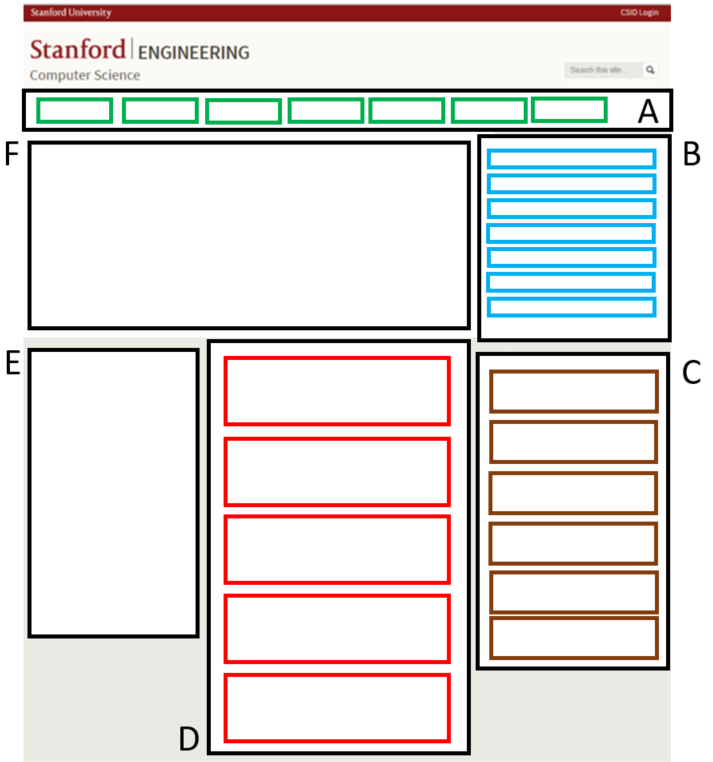
\includegraphics[scale=0.45]{imgs/chap_3/StanfordWebsiteBoxes}}\    
\subfloat[Structural Representation]
{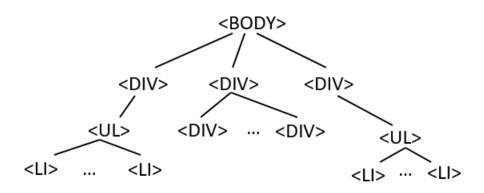
\includegraphics[scale=0.70]{imgs/chap_3/html}} 
\subfloat[Rendered Box Tree]
{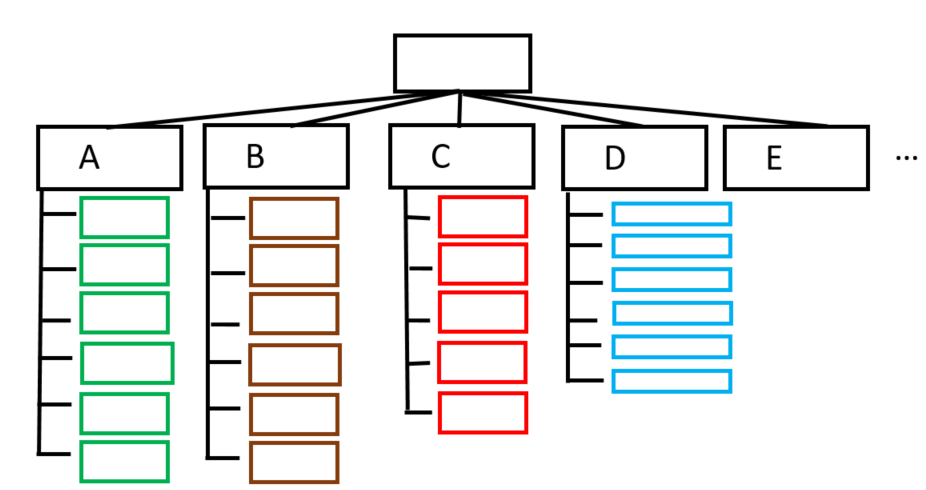
\includegraphics[scale=0.35]{imgs/chap_3/boxTree}}

\caption{}
\label{fig:Stanford}
\end{figure*}


Another important source of information proposed approach uses is the hyperlink structure of the website, which is formally introduced by the following definition:


\begin{definition}\label{def:website}A \textbf{Website} is a directed graph $G = (V, E)$, where $V$ is the set of web pages and $E$ is the set of hyperlinks. In most cases, the homepage $h$ of a website represents the website's entry page and, thus, allows the website to be viewed as a rooted directed graph. 
\end{definition}



As anticipated, the algorithm for the automatic identification of sitemaps exploits a sequential pattern mining step. The main  rationale behind this choice is to see a navigation path in a website as a sequence of urls and use sequences of urls to identify common (and frequent) navigation paths. Formally, a sequence is defined as follows:


\begin{definition}\label{def:sequence}\textbf{Sequence}:
Let $G = (V, E)$ be a website, a sequence $S$ is defined as $S=\langle t_1,t_2,\ldots,t_m \rangle$, where each item $t_j \in V$ denotes the web page at the $j$-th step in the navigation path $S$.
\end{definition}

A sequence $S=\langle t_1,t_2,\ldots,t_m \rangle$ is a \textbf{sub-sequence} of a sequence $S'=\langle a_1,a_2,\ldots,a_n \rangle$, if and only if integers $i_1, i_2, \dots, i_m$ exist, such that $1 \leq i_1 < i_2 < \dots < i_m \leq n$ and $t_1 = a_{i1}, t_2 = a_{i2}, \dots t_m = a_{im}$. We say that $S'$ is a \textbf{super-sequence} of $S$ or that $S'$ contains $S$.
\begin{example}
The sequence $S' = \langle a, b, d \rangle$ is a super-sequence of $S = \langle a,d \rangle $. On the contrary, $S'$ is not a super-sequence of $S'' = \langle e \rangle $, since the item $e$ is not equal to any item of $S'$.
\end{example}
Given a database of sequences $SDB$ and a single sequence $S$ the \emph{absolute support} of $S$ in $SDB$ is the number of sequences in $SDB$ which contain $S$, while its \emph{relative support} is the absolute support divided by the size of database (i.e., $|SDB|$).
With the term support I will refer to the relative support, unless otherwise specified:

\begin{equation}
\sigma(S) = \frac{|\{t \in SDB: S \textit{ is a  sub-sequence of } t\}|}{|SDB|}
\end{equation}

\noindent
A sequence is frequent if its support is greater than a user defined threshold. In our case the support defines the relationship strength among web pages.


Following the suggestion provided in \cite{Mobasher:2007}, we also exploit the definition of contiguous sequence which is formally defined as follows:

\begin{definition}\label{def:contiguousSeq}\textbf{Contiguous Sequence}: Given a sequence $S=\langle t_1,t_2,\ldots,t_m \rangle$ created from $G=(V,E)$, $S$ is contiguous if each item $t_i$ appears in $G$ contiguously to item $t_{i-1}$ (i.e. there is an edge between $t_{i-1}$ and $t_{i}$). 
\end{definition}


% Given a database of sequences $SDB$ and a single contiguous sequence $S$, the relative support of $S$ is defined as follows:
% \begin{equation}
% \sigma_{c}(S) = \frac{|\{t \in SDB: S \textit{ is a contiguous subsequence of } t\}|}{|SDB|}
% \end{equation}

The task of sequential pattern mining indicates the task of discovering frequent (sub-)sequences (contiguous sequences) from $SDB$. This is considered computationally challenging because  algorithms have to generate and/or test a combinatorially explosive number of intermediate sub-sequences. For this reason, we consider the simpler problem (in terms of time complexity) of identifying \textit{closed} sequential patterns which are compact and provide a lossless representation of all sequential patterns. A closed sequential pattern (or, simply, a closed sequence) is defined as follows:

\begin{definition}\label{def:closedSeq}\textbf{Closed Sequence}: %Given two sequences (contiguous sequences) $S_i$ and $S_j$, if $S_i$ is a supersequence of $S_j$ and their support in $SDB$ is the same, we say that $S_i$ absorbs $S_j$. 
A sequential pattern (contiguous sequential pattern) $S_j$ is \textbf{closed} if and only if it is frequent and its support is different from all of its frequent super-sequences.
\end{definition}
\begin{example}
Figure \ref{fig:myfigs}(b) shows an example of a database of sequences. Sequence $\langle h \rangle$ is closed because no super-sequences of $\langle h \rangle$  with the same support exist. 
On the contrary, the sequence $\langle h, d \rangle$ is not closed because the super-sequence $\langle h, b, d \rangle$ has the same support of $\langle h, d \rangle$.
\end{example}
\noindent



The last definition we have to provide before discussing technical details of the method is that of sitemap. This definition is particularly important since it defines the goal of the proposed method.



\begin{definition}\label{def:sitemap}\textbf{Sitemap}:
Given a web graph $G = (V,E)$ where $h\in V$ is the homepage, a user-defined threshold $t$ and a weight function $w:~E~\rightarrow~\mathbb{R} $, then $T = \argmax_{{T_i}}{\Phi(T_i)}$ is a sitemap if:
\begin{enumerate}
\item $T_i= (V_i',E_i')$ is a tree rooted in $h$, where $V_i' \subseteq V$ and $E_i' \subseteq E$;
\item $ \Phi(T_i) = \sum_{e \in E_i'} w(e)$;
\item  $\forall~e = (j_1,j_2) \in E_i', j_2 \in webList(j_1)$, that is, the url of the web page $j_2$ is contained in some \textit{web list} of the web page $j_1$ (See Def. \ref{def_chap2:list}); 
\item $\forall e \in E_i',~w(e) \geq t$. 
\end{enumerate} 
\end{definition}


\noindent

What remains unspecified in this (general) definition is the meaning of $w(\cdot)$ and the way the tree $T$ is generated. These aspects are discussed in the following section where we describe the method and instantiate aspects intentionally kept as parameters in Definition \ref{def:sitemap}.
We only anticipate that our solution does not need to enumerate all possible trees $T_i \subseteq G$ to optimize $\Phi(\cdot)$, yet it is able to extract directly $T$ analyzing a sub-graph of the website.

\section{Methodology}
\label{sec:methodology}


The problem we consider is that extracting the website's sitemap, defined according to Definition \ref{def:sitemap}. To achieve this goal, I combine different techniques which have roots in  web and data mining research areas: \emph{i)} Information extraction for identifying potential navigation systems in web pages in form of web-lists; \emph{ii) } Random Walk theory to extract navigation paths; \emph{iii)} Sequential pattern mining for finding the most frequent paths which describe the hierarchical structure of the website. 


In the first step of the proposed methodology we perform website crawling. Crawling uses web pages' structural and visual information to extract web lists in order to mitigate problems coming from noisy links. 
The output of this phase is the website graph $G$, where each node represents a single page and edges represent hyperlinks. Details of this step are described in Section~\ref{3Crawling}.
In the second phase we generate sequences of urls (i.e., web pages), which describe navigation paths. This is done by exploiting random walks extracted from the crawled website's graph. In the third phase we mine closed frequent sequences of urls (i.e., closed frequent navigation paths) in form of a tree.
In the last step the tree of closed sequences is analyzed in order to extract the sitemap. This step requires the transformation of the tree of sequences in a tree of web pages such that the obtained tree has the homepage as root and a web page appears only once, that is, it is not possible to have multiple paths that connect the homepage with a web page. 

% Finally, in the last phase is applied a pruning step to filter, for each node $v \in V'$, the best path which connect the homepage to $v$. The extracted tree is the website sitemap.


\subsection{Sequence Database Generation}
\label{dbGeneration}

To capture and codify correlations among graph's nodes (i.e. web pages) I use the Random Walk with Restart from Homepage (RWRH) approach. It can be considered a 
particular case of Random Walk with Restart, obtained setting a single node (i.e. the homepage) as starting vertex. Random walk with restart is widely adopted in several works to infer structural properties of nodes in a graph through the analysis of the global structure of the whole network.

Using this approach, web pages closer to the homepage have higher probability to be reached than those at deeper levels. %Moreover, the random walker with restart assigns higher probabilities to web pages closer to the homepage than those at deeper levels. 
This is coherent with the organization typically followed in the website navigation where navigation systems closer to the homepage belong to shallower levels of the website hierarchy.

Therefore, given the web graph $G$ extracted in the previous step, and two number $rwrLength, dbLength \in  \mathbb{N} $, the random walk theory is used to navigate the web graph $G$ from the homepage $h$. 
The output of this phase is a sequence database $SDB$ composed by $dbLength$ random walks having length $rwrLength$ and starting from $h$. As defined in \cite{Pons:2006}, increasing the length $rwrLength$ of a random walk starting at node $i$, the probability to reach a node $j$ tends to depend on the degree of $j$. As suggested in \cite{Pons:2006} we generate short random walks in the way that the random walker tends to get "trapped" into densely connected parts of the graph corresponding to communities (i.e. sibling pages in the sitemap) and for avoiding to infer false correlations among web pages due the nodes' degree.
Algorithm~\ref{3alg:datasetGeneration} describes the generation process of the sequence dataset.
Figure~\ref{fig:SDB} shows a sequence database obtained from the web graph in Figure~\ref{fig:graph}


\begin{algorithm}[tb]
\caption{rwrGeneration(rwrLength, dbLength, G, $\alpha$)}
\label{3alg:datasetGeneration}
\begin{algorithmic}[1]
\renewcommand{\algorithmicrequire}{\textbf{Input:}}
\newcommand{\RETURN}[1]{\textbf{return} #1}
\renewcommand{\algorithmicensure}{\textbf{Output:}}
\renewcommand{\algorithmiccomment}[1]{$//$ \textit{#1}}
\renewcommand{\algorithmicforall}{\textbf{for each}}
\newcommand{\getRandomVertex}[1]{ \textit{getRandomVertex}(#1); }
\newcommand{\getNextRandomVertex}[1]{ \textit{getRandomOutlink}(#1); }
\newcommand{\add}[1]{ \textit{add}(#1); }

\REQUIRE int rwrLength, int dbLength, Graph G, float $\alpha$;
\ENSURE List$<$List$<$URL$>>$ randomWalks;
	\FORALL{i $\in$ Range(0, dbLength)}
	    \STATE w = List()
	    \STATE w[0] = G.homepage
		\FORALL{j $\in$ Range(1, rwrLength) }
		\STATE $\lambda$ = Math.random()
		\IF{$\lambda > \alpha$}
		\STATE w[j] = G.\getNextRandomVertex{w[j-1]}
		\ELSE 
		\STATE w[j] = w[0]
		\ENDIF
		\ENDFOR
		\STATE randomWalks.\add{w}
 	\ENDFOR
\RETURN randomWalks

\end{algorithmic}
\end{algorithm}
  
%For this reason, we generate short random walks, in the way that the random walker tends to get “trapped” into densely connected parts of the graph corresponding to communities and to avoid the effect predicted in \cite{Pons:2006}.
%it is be too influenced by nodes degree .

\subsection{Closed sequential patter mining}
Given the sequence database (SDB), extracted in the Section~\ref{dbGeneration}, and a user defined threshold $t$ (i.e. minimum support), we apply a closed sequential pattern mining algorithm to extract all the frequent sequences. In this phase we used the algorithm CloFAST~\cite{Fumarola:2015} as closed sequential pattern mining algorithm. It  showed to provide compact results, saving computational time and space if compared with other closed sequential pattern mining algorithms.
CloFast returns a tree $T_{CloFAST} = (V', E')$ and a weight function $\sigma : E' \rightarrow \mathbb{R} $ which associates each edge $e=(j_1,j_2)\in E'$  with the \textit{relative} support of the sequence $\langle h, \ldots, j_1,j_2\rangle$ in $T_{CloFAST}$.

Figure~\ref{3fig:tree1} shows an example of tree extracted by CloFAST for the input sequence dataset in figure~\ref{3fig:sf1}. 

\begin{figure*}
\center
\subfloat[]{
\label{3fig:tree1}
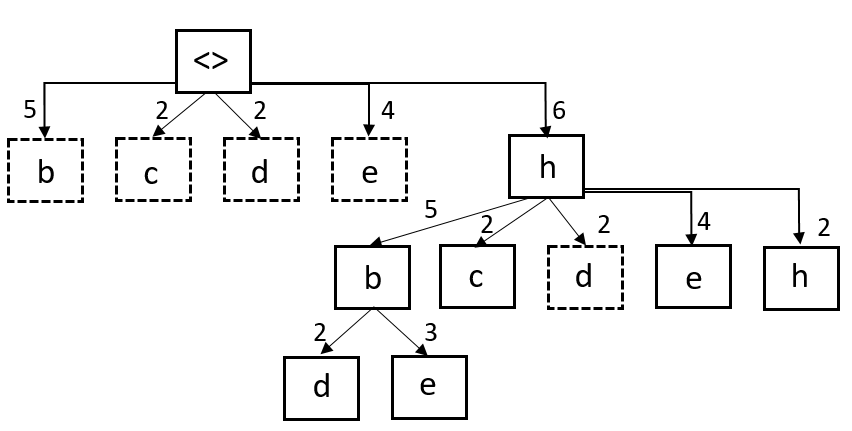
\includegraphics[scale=0.45]{imgs/chap_3/clofast}} \
\subfloat[]{
\label{3fig:tree2}
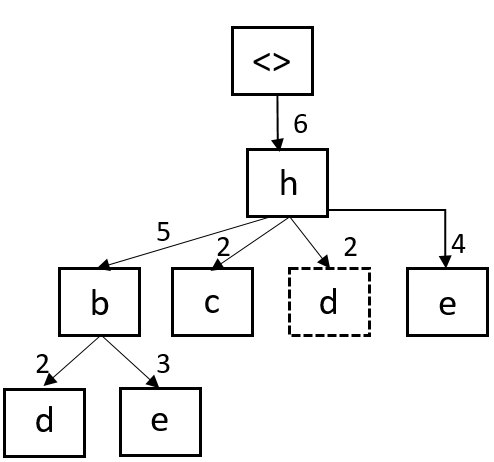
\includegraphics[scale=0.45]{imgs/chap_3/clofastPruned}}
\subfloat[]{
\label{3fig:tree3}
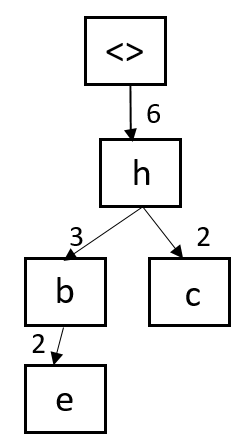
\includegraphics[scale=0.45]{imgs/chap_3/clofastContiguous}}
\caption{(a) Frequent sequence tree extracted by CloFAST with absolute minsup = 3 and SDB in fig. \ref{fig:myfigs}(b). Nodes with
dashed borders represent non-closed nodes; (b) Frequent sequences tree extracted by extended version of CloFAST and having the support as weight function; (c) Contiguous sequences tree extracted by extended version of CloFAST and having the contiguous support as weight function.}
\label{3fig:clofast}
\end{figure*}

Since a contribution of this chapter is to compare the sitemaps extracted considering two different types of sequences (i.e. sequential patterns and contiguous sequential pattern), I extend CloFAST by allowing it to also extract contiuous sequential patterns. 

To extract the weighted tree of contiguous sequences from $T_{CloFAST}$ I benefit of the data structure, called \textit{Vertical id-List} (VIL) provided by CloFAST for support counting purpose and for extracting frequent sequences. In the following we give a brief definition of a VIL:
\begin{definition}[Vertical Id-list]
Let $SDB$ be a sequence database of size \emph{n} (i.e. $|SDB| = n$), $S_j \in SDB$ its j-th sequence ($j \in \{1,2,\ldots,n\}$), and $\alpha$ a sequence associated to a node of the tree, its \emph{vertical id-list}, denoted as $VIL_{\alpha}$, is a vector of size $n$, such that for each $j=1,\ldots,n$
\begin{displaymath}
VIL_\alpha[j] = \left\{ \begin{array}{ll}
\textrm{$[pos_{\alpha,1}, pos_{\alpha,2}, \ldots, pos_{\alpha,m}]$ }\ \ \ \ & \textrm{if $S_j$ contains $\alpha$}\\
null & \textrm{otherwise}
\end{array} \right.
\end{displaymath}
where \emph{$pos_{\alpha,i}$} is the end position of the $i$-th occurrence ($i\leq m$) of $\alpha$ in $S_j$. 
\end{definition}

\begin{example}
\label{ex:vil}
Figure \ref{3fig:VILhb} shows the $VIL$ of the sequence $\alpha = \langle h , b \rangle$. Values in $VIL_{\alpha}$ represent the end position of the occurrences of the sequence $\alpha$ in the sequences of Figure \ref{fig:SDB}. In particular, the first element (list with only value 2) represents the position of the first occurrence of web page $b$, after the web page $h$ (i.e. $b$ is the last item in $\alpha$), in the first sequence $S_1$. The second element is (list with values 2 and 4) the position of the first item $b$ (after $a$) in the sequence $S_2$.
The other values are respectively list with only value 3 (for sequences $S_3$), list with only value  2 (for $S_4$) \emph{null} (for $S_5$) and list with only value 3 (for $S_6$).  In particular, the fifth element is null since $\alpha$ is not present in $S_5$.
Finally, the support of $\alpha$ is the number of not null elements in $VIL_{\alpha}$, that is 0.71.
\end{example}
\begin{figure}[tb]
  \centering
  \subfloat[]{\label{3fig:sf0}
  	\centering
    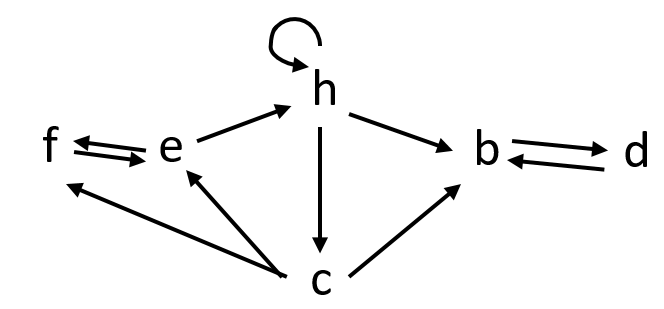
\includegraphics[scale=0.40]{imgs/chap_3/graph}
    \label{fig:graph}}
  \centering
  \subfloat[]{\label{3fig:sf1}
  	\centering
    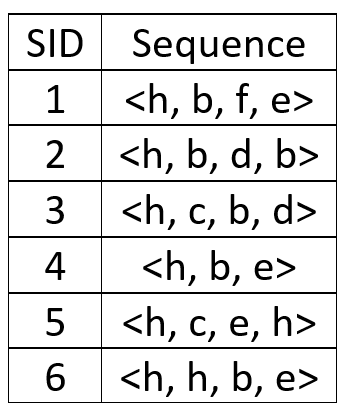
\includegraphics[scale=0.40]{imgs/chap_3/sequences.png}
    \label{fig:SDB}}
  \subfloat[]{\label{3fig:sf2}
  	\centering
  	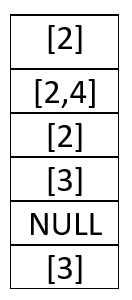
\includegraphics[scale=0.40]{imgs/chap_3/VILhb.png}
    \label{3fig:VILhb}}
  \caption{(a) Web Graph rooted at h; (b) Sequence Database (SDB), that is, a set of tuples (SID, Sequence), where SID is a sequence-id and Sequence is a random walk with restart from the homepage; (c) VIL for the sequence $\alpha = \langle h,b \rangle$.}
  \label{fig:myfigs}
\end{figure}
We modify the CloFAST implementation creating two pruning method that: \emph{i)} stop the generation of frequent sequences which start from a node different from the homepage; \emph{ii)} extract contiguous sequences. In particular, starting from the root of $T_{CloFAST}$, the function \textit{contiguous($\cdot$)} (see Algorithm~\ref{alg:contiguos}) is iteratively applied to update the node's VILs. It looks for possible holes in the sequences by botton-up clibing the sequence tree $T_{CloFAST}$. An hole is found when the condition at line 10 is not satisfied. Returned VIL of a node $n$ is used to calculate its contiguous support without scanning the sequence database SDB:
$\sigma_c(n) = \{j|vil = contiguous(n, T_{CloFAST}) \wedge  vil[j][1]= h\}$.
Therefore, if the contiguous support of $n$, $\sigma_c(n)$, is greater of the threshold $t$, the function is applied to its children, otherwise the node is pruned. We call the returned tree $T'_{CloFAST}$

\subsection{Sequence Pruning}
The trees $T_{CloFAST}$ (for sequential patterns) and $T'_{CloFAST}$ (for contiguous sequential patterns), extracted in the previous step, may contain multiple frequent paths to reach, from the homepage, a given node (web page). For example, in Figure~\ref{3fig:tree2} the web page $e$ can be reached using the frequent patterns $h\rightarrow b \rightarrow e$ and $h\rightarrow e$.
Since in the sitemap each web page can be reached by only one path starting from the homepage, the last task of the sitemap generation is the pruning process. Therefore, the goal of this step is to select for each web page included in the frequent sequence (contiguous sequence) tree, the best path to reach it.

A sequence  $\alpha = \langle u_1, \dots, u_i, u_{i+1}, \dots, u_n \rangle \in T_{CloFAST}$ is pruned if:
\begin{enumerate}
%\item $u_1 \neq h$, with $h$ the website's homepage;
\item $\nexists~(u_i, u_{i+1}) \in E$, with $1 \leq i < n$ and $u_1 = h$;
\item $\exists \beta = \langle h, \dots, u_n \rangle \in T_{CloFAST}$ ($T'_{CloFAST}$) and $\beta \neq \alpha$ such that 
\begin{equation}
\label{eq:pruning}
\sum_{e' \in T_{\beta}}w(e') + w(\beta) > \sum_{e \in T_{\alpha}}w(e) + w(\alpha)
\end{equation}
\end{enumerate}
%The first constraint prunes all frequent sequences which start from a node different from the homepage.
The first constraint ensures that frequent paths that do not exist in the crawled graph G are removed (see Def.~\ref{def:sitemap}.3).  The second constraint allows us to select for each node in $V'$ which can be reached by multiple frequent sequences, starting from the homepage, the best path. 
 In particular, for each node $u_n$, ending node of multiple frequent sequences (e.g. $\alpha$ and $\beta$), we compare all the sub-trees of $T_{CloFAST}$ ($T'_{CloFAST}$) having $u_n$ as root (e.g. $T_\alpha$ and $T_\beta$). From them, we only keep that one which maximize the sum of its edges plus the weight of the path starting from \emph{h} and reaching $u_n$ (e.g. $w(\alpha)$ and $w(\beta)$). For the case of sitemap extraction using sequential patterns we associate to the weight function $w(\cdot)$, defined in Def.~\ref{def:sitemap}, the support function $\sigma(\cdot)$ returned by CloFAST. For the case of sitemap extraction using contiguous sequential patterns we associate to $w(\cdot)$ the contiguous support function $\sigma_c(\cdot)$ calculated by Algorithm~\ref{alg:contiguos}. 

\begin{algorithm}[tb]
\begin{algorithmic}[1]
\renewcommand{\algorithmicrequire}{\textbf{Input:}}
\renewcommand{\algorithmicensure}{\textbf{Output:}}
\newcommand{\RETURN}[1]{\textbf{return} #1}
\renewcommand{\algorithmiccomment}[1]{$//$ \textit{#1}}
\newcommand{\getPos}[1]{ \textit{getPos}(#1); }
\newcommand{\length}[1]{ \textit{length}(#1); }
\newcommand{\shift}[1]{ \textit{next}(#1); }
\newcommand{\getVil}[1]{ \textit{getVil}(#1); }
\newcommand{\getParent}[1]{ \textit{getParent}(#1); }
\REQUIRE $T$: a sequence tree extracted by CloFAST; n: node of $T$
\ENSURE vil: the VIL of the sequence at node n such that the contiguous condition is satisfied.

\STATE vil = \getVil{n}
\STATE parent = \getParent{n}
\REPEAT 

	\STATE parentVil = \getVil{parent}
	\FORALL{ $j = 1 \ldots$\length{vil}}
		\STATE i=0; 	contiguous =  $FALSE$;
		\REPEAT
				\STATE z=0;
				\REPEAT
				\IF{ vil[j][i] = parentVil[j][z]+1 }
					\STATE vil[j] = parentVil[j][z..(len(parentVil[j])-1)];
					\STATE contiguous = $TRUE$ ;
				\ENDIF
			\UNTIL{$++z \leq i $ AND !contiguous}
			\IF{!contiguous}
				\STATE vil[j] = $NULL$\;				
			\ENDIF
		\UNTIL{$++i < len(vil[j])$ AND !contiguous }
	\ENDFOR
\STATE n = parent
\STATE parent = \getParent{n}\;
\UNTIL{parent != root(T)}
\RETURN vil;
\caption{contiguous(T,n)}
\label{alg:contiguos}
\end{algorithmic}
\end{algorithm}




\section{Experiments and Discussion}
\label{sec:experiments}
The aim of this chapter is to answer to the following research questions: 1) Which is the real contribution of combining the random walk teory with structured data with respect to use the content and the whole hyperlink structure? 2) Which is the real contribution of extracting hierarchies based on  sequential patterns with respect to extract hierarchies based on $contiguous$ sequential patterns. 
For this reason we compare the performances of SMAP (i.e. sitemap generation through sequential patterns) and $SMAP_{sc}$ (i.e. sitemap generation through $contiguous$ sequential patterns) with a state-of-art algorithm, that is HTDM~\cite{Weninger:2012}.

The empirical evaluation of these algorithms was not a trivial task because, at the best of our knowledge, there is no dataset generated for the specific task of sitemap extraction. 
Thus, two solutions were possible: \emph{i)} involving human experts to extract the hierarchical organization of websites and generating a ground truth dataset for each considered website; \emph{ii)} using existing sitemap pages, which are manually generated by web masters and provided by some website, as ground truth. 


In the first case, the involvement of experts requires extensive human effort and working time. This is not feasible in the context of the Web especially for websites having a great amount of web pages strongly connected and websites having deep hierarchies. In the second case, sitemap pages are in general manually created by web designers. Therefore, the risk is that sitemap pages are not updated (i.e. they can contain links to non-existent pages or they ignore the existence of new sections) or are very abstract (i.e. contain shallow hierarchies composed by few pages). For this reason, to empirically evaluate SMAP, I have performed experiments on following websites which provide updated sitemap pages: \emph{cs.illinois.edu}, \emph{www.cs.ox.ac.uk}, \emph{www.cs.princeton.edu}, and \emph{www.enel.it}. 

The evaluation has been performed in terms of Precision, Recall and F-measure of edges. In particular, the Precision measures how many of the extracted edges belong to the real sitemap. The Recall measures how many edges, belonging to the real sitemap are extracted.
%the discovered edges are true positive elements of the real sitemap.
I also included the F-Measure which is the weighted harmonic means of Precision and Recall. These measures are evaluated counting how many edges of the real sitemap are found by the algorithm under analysis (i.e. SMAP, $SMAP_{cs}$, HDTM).
More formally:


\begin{equation}
Precision= \frac{|\{e| e\in SMAP(G) \wedge e\in GT\_Sitemap \}| }{|\{e| e\in SMAP(G) \}| }
\end{equation} 

\begin{equation}
Recall=\frac{|\{e| e\in SMAP(G) \wedge e\in GT\_Sitemap \}| }{|\{e| e\in GT\_Sitemap \}| }
\end{equation} 


\begin{equation}
F = \frac{2(precision \times recall)}{precision + recall}
\end{equation} 

\noindent In these formulas $SMAP(G)$ represents the set of edges extracted by $SMAP$, whereas $GT\_Sitemap$ represents the set of edges in the real sitemap (ground truth).



%We analyzed the effectiveness of proposed approach (SMAP) with four real websites: \textit{cs.illinois.edu, www.cs.ox.ac.uk, www.cs.princeton.edu}, and \textit{www.enel.it}.  Each analyzed website contains a sitemap provided by the website's organization which allows us to have a ground truth and evaluate the extracted sitemaps in terms of precision, recall and F-measure of edges.
%The results are compared with those obtained by HDTM~\cite{Weninger:2012}. For HDTM  we set $\gamma = 0.25$ (to avoid too shallow or too deep hierarchies) and $5,000$ Gibbs iterations, as suggested by the authors in their paper. 
Table \ref{tableResSitemap} presents the main results. For HDTM  I set $\gamma = 0.25$ (to avoid too shallow or too deep hierarchies) and $5,000$ Gibbs iterations, as suggested by the authors in their paper. For SMAP and $SMAP_{cs}$ I set $rwrLength =10 $ and $dbLength=500.000$ (See Section \ref{dbGeneration}). Moreover, I analyze the effectiveness of SMAP and $SMAP_{cs}$ varying the minimum support. It is interesting to note that when the minimum support threshold decreases, we are able to obtain deeper and wider sitemaps. While, as expected, by reducing the minimum support threshold, precision increases and recall decreases. 
This is due to the fact that, by decreasing the support, the number of generated sequences increases and the extracted hierarchy becomes deeper and wider, including website sections which are not included in the sitemap page. This behaviour can be observed by analyzing the F-measure which, from website to website, shows different trends for different values of minimum support.

Interestingly, both versions of our algorithm significantly outperform HDTM, independently of the website and of the minimum support threshold. 
This can be motivated by the different nature of the two algorithms: on the contrary of our approach, HDTM organizes website's pages in a hierarchy using the distribution of web pages' terms. Then, it can happen that, for example, for a Computer Science department website HDTM organizes the web page of a \emph{professor} as a child of its \emph{research area} web page rather than as a child of the \emph{professors} web page. In this way, web pages clustered together as siblings in the hierarchy by web masters are split in different parts of the extracted hierarchy.

Finally comparing the sitemaps extracted using sequential patterns and $contiguous$ sequential patterns we can observe that in general SMAP outperforms $SMAP_{sc}$. This is due by the fact that $SMAP_{sc}$ extracts narrower and shallower hierarchies compared with $SMAP$. In fact, setting low support thresholds $SMAP_{sc}$ obtain better results than SMAP in terms of Recall but, since it is unable to extract the deepest levels, it obtains lower results in terms of Precision.

%What is interesting is that F-measure depends on the website and, more precisely, on the level of details of the ground truth (real sitemaps). 

\begin{table}[t]

\centering

\begin{tabular}{|c|c|c|c|c|c|}
\hline
Website & Algorithm & min. supp. & Precision & Recall & F-Measure  \\
\hline
cs.illinois.edu & SMAP & 0.005  & 0.38 & \textbf{0.78} & 0.51 \\
cs.illinois.edu & $SMAP_{cs}$ & 0.005  &0.1	& 0.65	& 0.17 \\
cs.illinois.edu & SMAP & 0.001  & 0.66 & 0.48 & \textbf{0.56} \\
cs.illinois.edu & $SMAP_{cs}$ & 0.001  & 0.35& 0.76 & 0.48  \\
cs.illinois.edu & SMAP & 0.0005 & 0.66 & 0.33 & 0.44 \\
cs.illinois.edu & $SMAP_{cs}$ & 0.0005  & 0.35 & 0.33  & 0.34  \\
cs.illinois.edu & SMAP & 0.0001 & \textbf{0.75} & 0.26  & 0.38 \\
cs.illinois.edu & $SMAP_{cs}$ & 0.0001  & 0.61 & 0.35  & 0.45  \\
cs.illinois.edu & HDTM & $-$ &  0.12 & 0.1 & 0.11 \\
\hline
cs.ox.ac.uk &  SMAP & 0.005  & \textbf{0.72} & 0.3 & \textbf{0.42} \\
cs.ox.ac.uk &  $SMAP_{cs}$ & 0.005  & 0.27 & \textbf{0.41} & 0.33 \\
cs.ox.ac.uk &  SMAP & 0.001 & \textbf{0.72} & 0.21 & 0.33 \\
cs.ox.ac.uk &  $SMAP_{cs}$ & 0.001  & 0.60& 0.18 &1.28  \\
cs.ox.ac.uk &  SMAP & 0.0005  & 0.72 & 0.21 & 0.33 \\
cs.ox.ac.uk &  $SMAP_{cs}$ & 0.0005  & 0.60& 0.17 &0.27  \\
cs.ox.ac.uk &  SMAP & 0.0001  & \textbf{0.72} & 0.21 & 0.33 \\
cs.ox.ac.uk &  $SMAP_{cs}$ & 0.0001  & 0.60& 0.17 &0.27  \\
cs.ox.ac.uk &  HDTM & $-$ & 0.37 & 0.15 & 0.21 \\
\hline
cs.princeton.edu &  SMAP & 0.005  & 0.61 & \textbf{0.55} & \textbf{0.58} \\
cs.princeton.edu &  $SMAP_{cs}$ & 0.005  & 0.1& 0.22 & 0.14 \\
cs.princeton.edu &  SMAP & 0.001  & 0.89 & 0.23 & 0.36 \\
cs.princeton.edu &  $SMAP_{cs}$ & 0.001  & 0.6&  0.55& 0.58 \\
cs.princeton.edu &  SMAP & 0.0005  & 0.89 & 0.2 & 0.33 \\
cs.princeton.edu &  $SMAP_{cs}$ & 0.0005  & 0.6 &0.32  &0.41  \\
cs.princeton.edu &  SMAP & 0.0001 & \textbf{0.9}1 & 0.13 & 0.23 \\
cs.princeton.edu &  $SMAP_{cs}$ & 0.0001  & 0.73 & 0.18 & 0.29  \\
cs.princeton.edu &  HDTM & $-$ & 0.36 & 0.08 & 0.13 \\
\hline
enel.it & SMAP & 0.005 & 0.31 & 0.74 & 0.43 \\
enel.it &  $SMAP_{cs}$ & 0.005  &0.1 & 0.47 & 0.16  \\
enel.it & SMAP & 0.001  & 0.36 & 0.72 & 0.48 \\
enel.it &  $SMAP_{cs}$ & 0.001  & 0.31& 0.73 & 0.43 \\
enel.it & SMAP & 0.0005  & 0.8 & 0.73 & 0.76 \\
enel.it &  $SMAP_{cs}$ & 0.0005  & 0.31 & 0.73  & 0.43  \\
enel.it & SMAP & 0.0001  & \textbf{0.8} & 0.73 & 0.76 \\
enel.it &  $SMAP_{cs}$ & 0.0001  & 0.77 & \textbf{0.8}  & \textbf{0.79}  \\
enel.it & HDTM & $-$ & 0.35 & 0.75 & 0.48 \\
\hline
\end{tabular}
\caption{Experimental results of SMAP, $SMAP_{cs}$ and HDTM.}
\label{tableResSitemap}
\end{table}